\documentclass[aspectratio=169,14pt]{beamer} % \documentclass[14pt]{beamer}
\maxdeadcycles=20
\usepackage[utf8]{inputenc}
\usepackage[english]{babel}
% \usepackage[brazil]{babel}
\usepackage[T1]{fontenc}
\usepackage{graphicx}
\usepackage{pax}
\usepackage{tikzscale}
\usepackage{appendix}
\usepackage{pgfplots}
\pgfplotsset{compat=newest}
\usepgfplotslibrary{groupplots}
\usepgfplotslibrary{dateplot}
\usepackage{xargs}
\usepackage{rotating}
\usepackage{pdflscape}
\usepackage{afterpage}
\usepackage[paper=A4,pagesize]{typearea}
\graphicspath{{../../figures/}} 
\usepackage{subcaption} 
\usepackage{hyperref}
\usepackage{amsmath,amssymb} 
\usepackage{indentfirst}
\usepackage[algo2e,linesnumbered,ruled]{algorithm2e}
\usepackage{algorithmic}
%%If desirable, the user can enable Times New Roman Fonts by uncommenting the next line. G.L.
% \usepackage{mathptmx}
\usepackage{pdfpages}
\usepackage{multirow}
\usepackage{color}
\usepackage{blindtext}
\usepackage{float}
\usepackage{nameref}
\usepackage{cleveref}
\usepackage{multicol}
\usepackage{listings}
\usepackage{enumerate}
\usepackage[acronym,toc]{glossaries}\makeglossaries
\usepackage{tikz}
\usepackage{ladder} %https://github.com/AurelienC/tex-ladder/blob/master/ladder.sty
\usetikzlibrary{arrows,shapes,automata,petri,external,arrows.meta}
	\tikzset{
	place/.style={
	circle,
	thick,
	draw=black!100, % draw=blue!75,
    % fill=blue!20,
    minimum size=6mm
  },
  extPlace/.style={
    circle,
    dotted,
    draw=black!100, % draw=blue!75,
    % fill=blue!20,
    minimum size=6mm
  },
  extTransition/.style={
    rectangle,
    dotted,
    fill=white,
    minimum width=8mm,
    inner ysep=0.7pt
  },
  transition/.style={
    rectangle,
    thick,
    fill=black,
    minimum width=8mm,
    inner ysep=0.7pt
  },
  extTimedtransition/.style={
    rectangle,
    dotted,
    fill=white,
    minimum width=8mm,
    inner ysep=2pt
  },
  timedtransition/.style={
    rectangle,
    thick,
    fill=white,
    minimum width=8mm,
    inner ysep=2pt
  },
  inhibitor/.style={-o},
  text/.style={}
}

\makeatletter
\tikz@def@grow@tokens{2}{1}{-1.5}{0}
\tikz@def@grow@tokens{2}{2}{1.5}{0}
% \tikz@def@grow@tokens{3}{1}{-1}{0}
% \tikz@def@grow@tokens{3}{2}{0}{1}
% \tikz@def@grow@tokens{3}{3}{1.5}{-1}
\makeatother


\definecolor{darkblue}{rgb}{0,0,0.3}
\definecolor{blue}{rgb}{0,0,0.5}
\definecolor{color1}{rgb}{1,0.2,0.3}
\definecolor{color2}{rgb}{0.05490196078,0.41176470588,0.13333333333}
% rgb(14, 105, 34)

\definecolor{color3}{rgb}{0.2,0.2,0.8}
% hyperref setup
\hypersetup{
  % pdftitle={\title},
  pdfauthor={Rafael Accácio Nogueira},
  pdfcreator={Rafael Accácio Nogueira},     
  bookmarksopen=true,         
  bookmarksopenlevel=1,       
  colorlinks=true, % false => boxes 
  linkcolor=blue,
  filecolor=red,  
  urlcolor=blue,  
  citecolor=blue,              
  pdfstartview=Fit,          
  pdfpagemode=UseOutlines,    % this is the option you were lookin for
  pdfpagelayout=TwoPageRight,
}

\makeatletter
\let\stdchapter\chapter
\renewcommand*\chapter{%
  \@ifstar{\starchapter}{\@dblarg\nostarchapter}}
\newcommand*\starchapter[1]{\stdchapter*{#1}}
\def\nostarchapter[#1]#2{
  \stdchapter[#1]{\protect\hyperlink{tocsection}{#1}}}
\makeatother

\makeatletter
\let\stdsection\section
\renewcommand*\section{%
  \@ifstar{\starsection}{\@dblarg\nostarsection}}
\newcommand*\starsection[1]{\stdsection*{#1}}
\def\nostarsection[#1]#2{
  \stdsection[#1]{\protect\hyperlink{tocsection}{#1}}}
\makeatother

\makeatletter
\let\stdsubsection\subsection
\renewcommand*\subsection{%
  \@ifstar{\starsubsection}{\@dblarg\nostarsubsection}}
\newcommand*\starsubsection[1]{\stdsubsection*{#1}}
\def\nostarsubsection[#1]#2{
  \stdsubsection[#1]{\protect\hyperlink{tocsection}{#1}}}
\makeatother

\makeatletter
\let\stdsubsubsection\subsubsection
\renewcommand*\subsubsection{%
  \@ifstar{\starsubsubsection}{\@dblarg\nostarsubsubsection}}
\newcommand*\starsubsubsection[1]{\stdsubsubsection*{#1}}
\def\nostarsubsubsection[#1]#2{
  \stdsubsubsection[#1]{\protect\hyperlink{tocsection}{#1}}}
\makeatother

\let\oldtoc\tableofcontents
\renewcommand{\tableofcontents}{\pagebreak\hypertarget{tocsection}{}\label{tocsection}\oldtoc}


\newcommand{\figplaceholder}[2]{
	\begin{figure}[H]
		\begin{center}	
			\rule{8cm}{8cm}
			\caption{\todo[FORGOT TO INCLUDE FIGURE]{#1 (placeholder)}}
			\label{fig:#2}
		\end{center}
	\end{figure}
}

\newif\ifdebug
\newcommand{\draft}{\debugtrue}
\newcommand{\final}{\debugfalse}
\newcommand{\todo}[2][FORGOT TO DO SOMETHING]{\ifdebug {\color{red}#2}\else \PackageError{}{#1}{}\fi}
\newcommand\doing[1]{\ifdebug {\color{blue}#1}\else \PackageError{}{FORGOT TO DO SOMETHING}{}\fi}
\newcommand\warning[1]{\ifdebug {\color{red}#1}\fi}
\newcommand\note[1]{\ifdebug {\color{orange}#1}\fi}

\usepackage{fancyhdr}
\pagestyle{fancy}

\fancyhead[L]{\warning{DRAFT}}
\fancyhead[R]{\warning{DEBUG ON}}

\fancyfoot[L]{\warning{TURN DEBUG OFF}}
\fancyfoot[R]{\warning{DRAFT}}

\newtheorem{theorem}{Theorem}
\numberwithin{theorem}{chapter}

\newtheorem{example}{Example}
\numberwithin{example}{chapter}

\newtheorem{definition}{Definition}
\numberwithin{definition}{chapter}

\newtheorem{observation}{Remark}
\numberwithin{observation}{chapter}

\usepackage[export]{adjustbox}

\newcommand{\includetikzfigure}[2][]{
    \ifdebug {\includegraphics[#1]{#2.pdf}}
    \else  \includegraphics[#1]{#2}\fi
}

\newcommand{\addtikzfigureLandscape}[4][width=0.8\textwidth]{
\KOMAoptions{paper=landscape}
\recalctypearea
  \vspace*{\fill}
  \begin{figure}[H]
    \centering
    \ifdebug {\includegraphics[#1]{#2.pdf}}
    \else  \includegraphics[#1]{#2}\fi
    \caption{#3}
    \label{fig:#4}
  \end{figure}
  \vspace*{\fill}
\KOMAoptions{paper=portrait}
\recalctypearea
}

\newcommand{\addtikzfigureLandscapeAthree}[4][width=0.8\textwidth]{
\KOMAoptions{paper=a3,paper=landscape}
% \KOMAoptions{paper=landscape}
\recalctypearea
  \begin{figure}[H]
    \vspace{-2cm}
    \centering
    \ifdebug {\centerline{\includegraphics[#1]{#2.pdf}}}
    \else  \centerline{\includegraphics[#1]{#2}}
\fi
    % \caption{#3}
    % \label{fig:#4}
  \end{figure}
\KOMAoptions{paper=a4,paper=portrait}
\recalctypearea
}

% \newcommand{\addtikzfigureVertCent}[3]{
% \KOMAoptions{paper=landscape}
% \recalctypearea
% % \begin{landscape}
% \vspace*{\fill}
%   \begin{figure}[H]
%     % \centering
%     % \resizebox{\hsize}{!}{
%     % \input{#1}
%      \includegraphics[width=1.15\textwidth]{#1}
%     % }
%     \caption{#2}
%     \label{fig:#3}
%   \end{figure}
% \vspace*{\fill}
% % \end{landscape}
% \KOMAoptions{paper=portrait}
% \recalctypearea
% }

\newcolumntype{P}[1]{>{\centering\arraybackslash}p{#1}}
\newcolumntype{M}[1]{>{\centering\arraybackslash}m{#1}}
\definecolor{keywordstyle}{rgb}{0,0,0.82}
\definecolor{commentstyle}{rgb}{0,0.6,0}
\definecolor{numberstyle}{rgb}{0.5,0.5,0.5}
\definecolor{stringstyle}{rgb}{0.58,0,0.82}

% Listing options
\lstset{ 
  % backgroundcolor=\color{white},   % choose the background color; you must add \usepackage{color} or \usepackage{xcolor}; should come as last argument
  basicstyle=\footnotesize,        % the size of the fonts that are used for the code
  breakatwhitespace=false,         % sets if automatic breaks should only happen at whitespace
  breaklines=true,                 % sets automatic line breaking
  captionpos=t,                    % sets the caption-position to bottom
  commentstyle=\color{commentstyle},    % comment style
  deletekeywords={...},            % if you want to delete keywords from the given language
  escapeinside={\%*}{*)},          % if you want to add LaTeX within your code
  extendedchars=true,              % lets you use non-ASCII characters; for 8-bits encodings only, does not work with UTF-8
  % firstnumber=1000,                % start line enumeration with line 1000
  % frame=single,	                   % adds a frame around the code
  keepspaces=true,                 % keeps spaces in text, useful for keeping indentation of code (possibly needs columns=flexible)
  keywordstyle=\color{keywordstyle},       % keyword style
  % language=Octave,                 % the language of the code
  morekeywords={*,...},            % if you want to add more keywords to the set
  numbers=left,                    % where to put the line-numbers; possible values are (none, left, right)
  numbersep=10pt,                   % how far the line-numbers are from the code
  numberstyle=\tiny\color{numberstyle}, % the style that is used for the line-numbers
  rulecolor=\color{black},         % if not set, the frame-color may be changed on line-breaks within not-black text (e.g. comments (green here))
  showspaces=false,                % show spaces everywhere adding particular underscores; it overrides 'showstringspaces'
  showstringspaces=false,          % underline spaces within strings only
  showtabs=false,                  % show tabs within strings adding particular underscores
  stepnumber=2,                    % the step between two line-numbers. If it's 1, each line will be numbered
  stringstyle=\color{stringstyle},     % string literal style
  tabsize=2,	                   % sets default tabsize to 2 spaces
  title=\lstname                   % show the filename of files included with \lstinputlisting; also try caption instead of title
}

%% as seen in https://tex.stackexchange.com/a/183682/143332
\makeatletter
\newcommand\Autoref[1]{\@first@ref#1,@}
\def\@throw@dot#1.#2@{#1}% discard everything after the dot
\def\@set@refname#1{%    % set \@refname to autoefname+s using \getrefbykeydefault
    \edef\@tmp{\getrefbykeydefault{#1}{anchor}{}}%
    \xdef\@tmp{\expandafter\@throw@dot\@tmp.@}%
    \ltx@IfUndefined{\@tmp autorefnameplural}%
         {\def\@refname{\@nameuse{\@tmp autorefname}s}}%
         {\def\@refname{\@nameuse{\@tmp autorefnameplural}}}%
}
\def\@first@ref#1,#2{%
  \ifx#2@\autoref{#1}\let\@nextref\@gobble% only one ref, revert to normal \autoref
  \else%
    \@set@refname{#1}%  set \@refname to autoref name
    \@refname~\ref{#1}% add autoefname and first reference
    \let\@nextref\@next@ref% push processing to \@next@ref
  \fi%
  \@nextref#2%
}
\def\@next@ref#1,#2{%
   \ifx#2@ and~\ref{#1}\let\@nextref\@gobble% at end: print and+\ref and stop
   \else, \ref{#1}% print  ,+\ref and continue
   \fi%
   \@nextref#2%
 }
 \makeatother

\newcommand{\colvec}[2][1]{%
  \scalebox{#1}{%
    \renewcommand{\arraystretch}{.7}%
    $\begin{bmatrix}#2\end{bmatrix}$%
  }
}


%%% Local Variables:
%%% mode: latex
%%% TeX-master: "./monografia.tex"
%%% End:

\usetheme[pageofpages=/,% String used between the current page and the
% total page count.
bullet=circle,% Use circles instead of squares for bullets.
titleline=true,% Show a line below the frame title.
alternativetitlepage=true,% Use the fancy title page.
titlepagelogo=poli-logo.pdf,% Logo for the first page.
watermark=polilogo_transp,% Watermark used in every page.
watermarkheight=0px,% Height of the watermark.
watermarkheightmult=0,% The watermark image is 4 times bigger
% than watermarkheight.
]{Torino}
\usefonttheme[onlymath]{serif}
\usecolortheme{blue}

\usefonttheme{serif}

\definecolor{lettercolor}{rgb}{0, 0,  0}
\setbeamertemplate{blocks}[rounded][shadow=false]







%%% Local Variables:
%%% mode: latex
%%% TeX-master: "presentation"
%%% End:

\author{\small \textbf{Rafael Accácio Nogueira}}
\title{\setlength\lineskip{10pt} \Large \textbf{Identificação de um Sistema de Manufatura Didático}}
\institute{}
\date{19 de Julho de 2019}
\usepackage[absolute,overlay]{textpos} %needed for textblock
\setbeamertemplate{navigation symbols}{} % don't use navigation tools on slides
\usepackage[timeinterval=60]{tdclock}
% \setbeameroption{show notes on second screen}
\setbeamertemplate{note page}{\pagecolor{white}\vfill\insertnote\vfill}
\makeindex


\begin{document}
\begin{frame}[t,plain]
	\titlepage
\end{frame}
%%% Local Variables:
%%% mode: latex
%%% TeX-master: "apresentation"
%%% End:
 
\setbeamertemplate{section in toc}[square]
\setbeamertemplate{subsection in toc}[square]
\newcommand{\eachsectiononlycurrentsubsections}{\AtBeginSection[]{
	\begin{frame}
	\frametitle{Sumário}
	%			\linespread{1.3}
	\tableofcontents[currentsection,sectionstyle=show/hide,subsectionstyle=show/show/hide]
\end{frame}
}}
\eachsectiononlycurrentsubsections

\begin{frame}{Sumário}\note{Falar o sumário}
% \begin{multicols}{2}
	\tableofcontents[subsectionstyle=hide/hide]
% \end{multicols}
\end{frame}
      
%%% Local Variables:
%%% mode: latex
%%% TeX-master: "presentation"
%%% End:

\newcommand{\bulletpoint}[1]{\begin{itemize}
		\item #1
\end{itemize}}

% \begin{frame}{Cycle}
% \centering
% \href{run:../../videos/TCCVIDEO_cycle.avi}{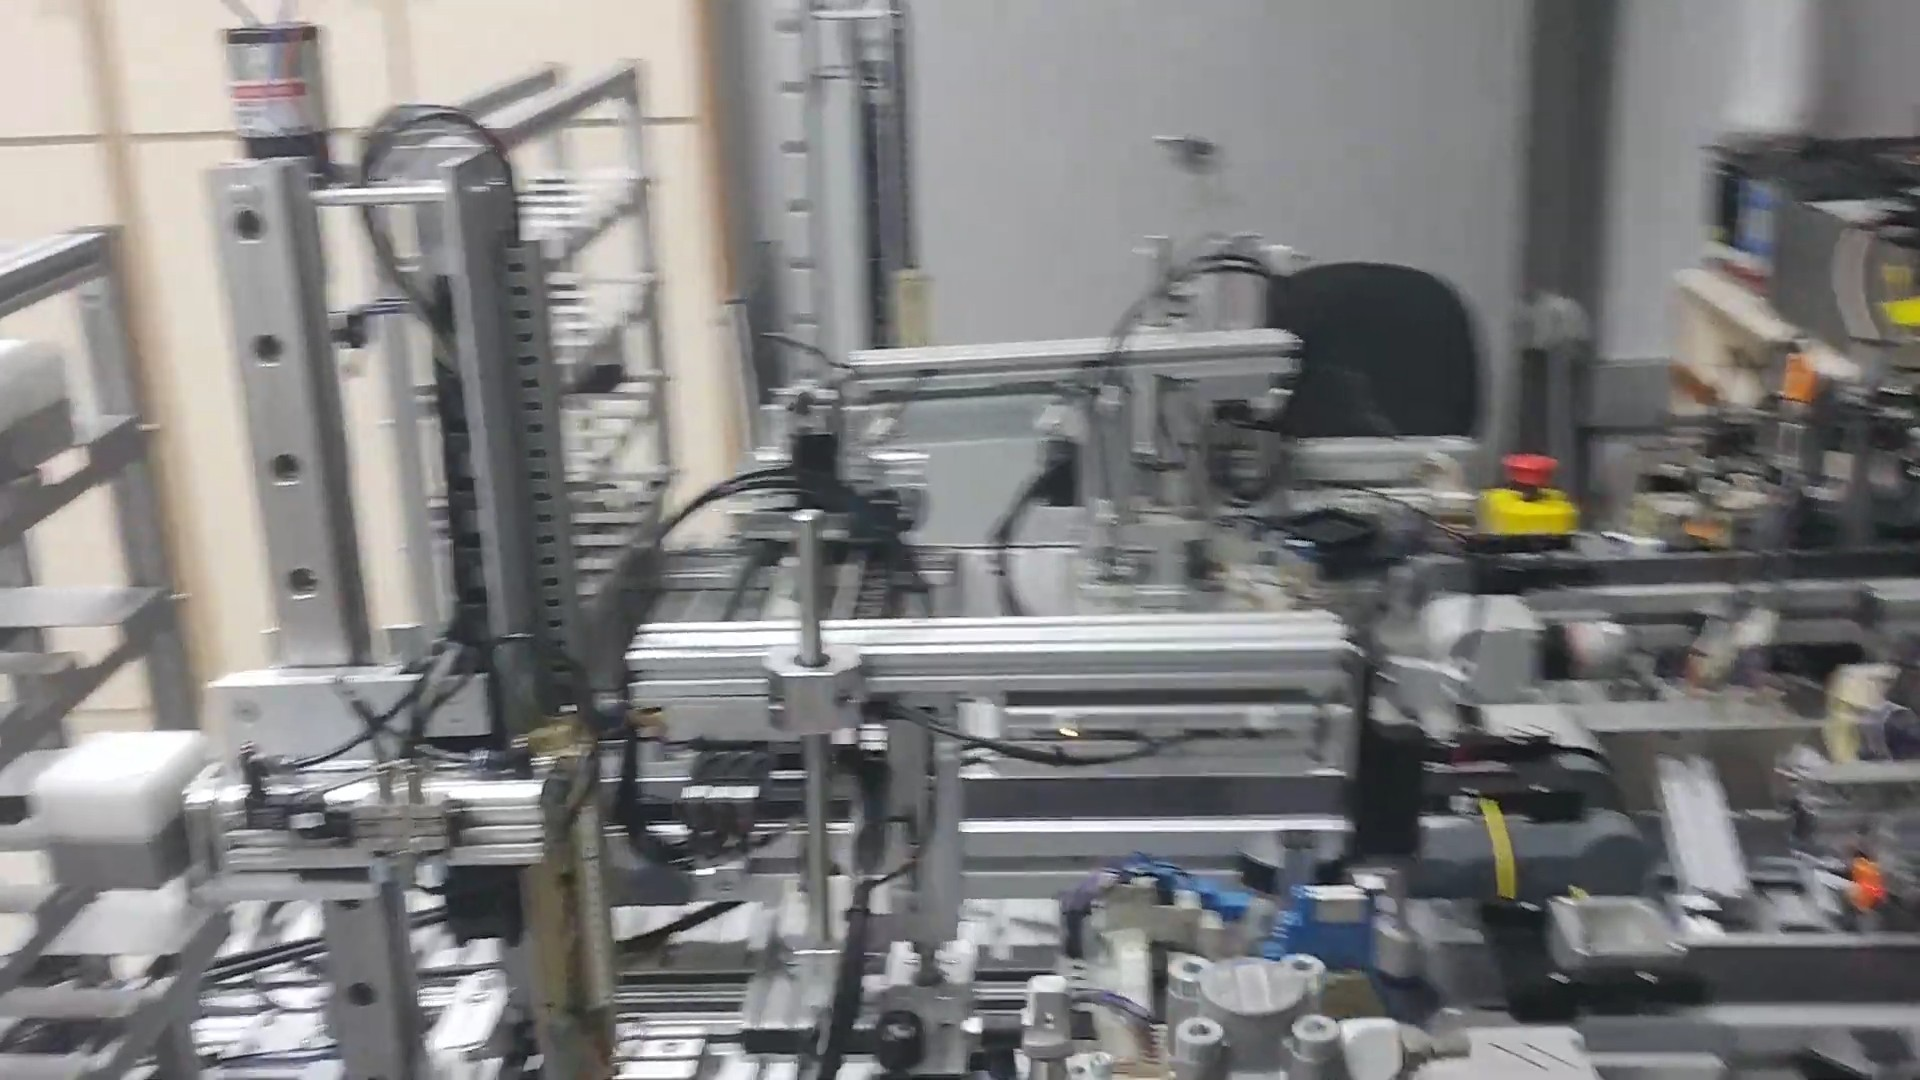
\includegraphics[width=0.7\textwidth]{../../videos/TCCVIDEO_cycle.jpg}}
% \note{Exemplo de }
% \end{frame}

% \begin{frame}{Teste}
% \centering
% \href{run:../../videos/TCCVIDEO_HTML-HTMI.avi}{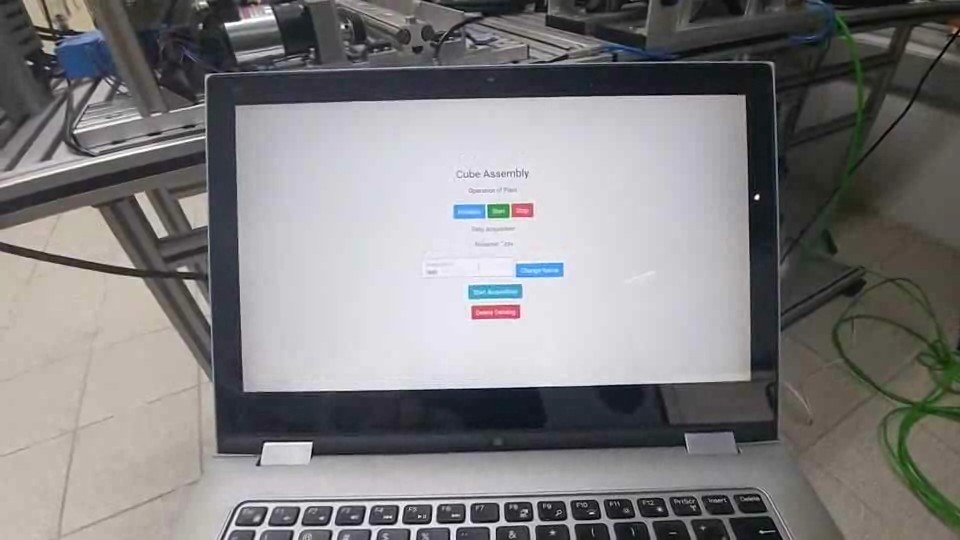
\includegraphics[width=0.7\textwidth]{../../videos/TCCVIDEO_HTML-HTMI.jpg}}
%  % \inlineMovie[]{../../videos/TCCVIDEO_HTML-HTMI.avi}{../../videos/TCCVIDEO_HTML-HTMI.jpg}{width=0.7\textwidth}
% \end{frame}
% \section{Title}
% \begin{frame}{Exemplo de frases espaçadas tipo Afonso}
% 	\onslide<1,2,3,5>{\quad First Line of Text}
% 	\only<2,3>{\\ \quad \quad Second Line of Text}
% 	\onslide<3>{\\ \quad \quad \quad Third Line of Text}
% \end{frame}

% \begin{frame}{Imagem}
% \begin{figure}
% 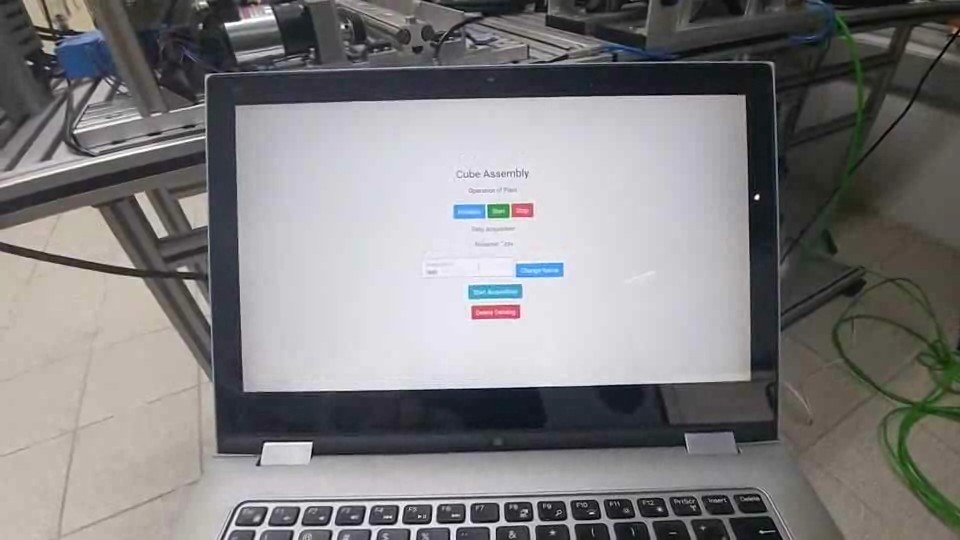
\includegraphics[height=4cm]{../../videos/TCCVIDEO_HTML-HTMI.jpg}
% \caption{Figura}
% \end{figure}
% \end{frame}
\begin{frame}{Rede de Petri}
\begin{figure}[H]
  \centering \includegraphics[width=0.8\textwidth]{cipnExample/schemePresentation.tikz}
  \caption{Exemplo de sistema a ser controlado.}
  \label{fig:cipnexamplescheme}
\end{figure}
\end{frame}
 
\begin{frame}{Rede de Petri}
\begin{figure}[H]
  \centering \includegraphics[width=\textwidth]{cipnExample/cipnPresentation.tikz}
  \caption{Exemplo de Rede de Petri interpretada para controle.}
  \label{fig:cipnexample}
\end{figure}
\end{frame}

\begin{frame}{Rede de Petri}
\begin{figure}[H]
 \sbox0{
   \includegraphics[width=0.5\textwidth]{vennDiagramLanguagesPresentation.tikz}
 }
  % \centering
 \begin{minipage}{1.2\wd0}
  \centering
   \usebox0
   \caption{Diagram de Venn com relações entre $L_{Orig}$, $L_{OrigNI}$,
    $L_{Obs}$, $L_{Exc}$ and $L_{Iden}$}.
 \end{minipage}
  \label{fig:languagesVenn}
\end{figure}
\end{frame}


\begin{frame}
\begin{definition}[DAOCT]
  \label{def:daoct}
  \small
  \[ DAOCT = (X,\Sigma,f,\lambda,R,\theta, x_0,X_f)\]
  \indent X conjunto de \textbf{estados} \\
  \indent $\Sigma$ conjunto de \textbf{eventos}\\
  \indent $\Omega \subset \mathbb{N}_1^{m_i+m_o} $ conjunto de \textbf{vetores E/S}\\
  \indent $f:  X \times \Sigma^\star \rightarrow X$ função de  \textbf{transição determinística}\\
  \indent $\lambda : X \rightarrow \Omega$ função de  \textbf{saídas do stado}\\
  \indent $R = {1,2,\dots,r}$ conjunto de \textbf{indices dos caminhos}\\
  \indent $\theta : X \times \Sigma \rightarrow 2^R$ função de \textbf{estimação
    de caminho}\\
  \indent $x_0$ \textbf{estado inicial} \\
  \indent $X_f \subseteq X $ conjunto de \textbf{estados finais}
\end{definition}
\end{frame}

\begin{frame}{Caminhos Observados}
  \setlength\arraycolsep{2pt}
  \vspace{-0.5cm}
\small \begin{align*}
  p_1&= \left(\colvec{1\\0\\0},a,\colvec{1\\1\\0},b,\colvec{0\\1\\1},c,\colvec{0\\0\\0},d,\colvec{0\\0\\1},e,\colvec{1\\0\\0}\right) \\
  p_2&= \left(\colvec{1\\0\\0},g,\colvec{0\\0\\0},h,\colvec{1\\1\\0},b,\colvec{0\\1\\1},c,\colvec{0\\0\\0},i,\colvec{1\\0\\0},j,\colvec{0\\1\\1},l,\colvec{1\\0\\0}\right) \\
  p_3&= \left(\colvec{1\\0\\0},g,\colvec{0\\0\\0},h,\colvec{1\\1\\0},b,\colvec{0\\1\\1},i,\colvec{1\\1\\1},m,\colvec{0\\0\\0},d,\colvec{0\\0\\1},n,\colvec{1\\1\\0}\right) \\
\end{align*}
\end{frame}

\begin{frame}{Caminhos Modificados}
  \setlength\arraycolsep{2pt}
 $\bullet$ $k=2$
 \small
 \begin{align*}
  p_1&= \left(\colvec{1\\0\\0},a,\colvec{1\\1\\0},b,\colvec{0\\1\\1},c,\colvec{0\\0\\0},d,\colvec{0\\0\\1},e,\colvec{1\\0\\0}\right)
\end{align*}
 \begin{align*}
  p_1^2&= \left(\colvec{1\\0\\0},a,\colvec{1&1\\0&1\\0&0},b,\colvec{1&0\\1&1\\0&1},c,\colvec{0&0\\1&0\\1&0},d,\colvec{0&0\\0&0\\0&1},e,\colvec{0&1\\0&0\\0&0}\right) \\ 
\end{align*}
\end{frame}

\begin{frame}{Caminhos Modificados}
  \setlength\arraycolsep{2pt}
 $\bullet$ $k=2$
  \small \begin{align*}
  p_1^2&= \left(\colvec{1\\0\\0},a,\colvec{1&1\\0&1\\0&0},b,\colvec{1&0\\1&1\\0&1},c,\colvec{0&0\\1&0\\1&0},d,\colvec{0&0\\0&0\\0&1},e,\colvec{0&1\\0&0\\0&0}\right) \\ 
  p_2^2&= \left(\colvec{1\\0\\0},g,\colvec{1&0\\0&0\\0&0},h,\colvec{0&1\\0&1\\0&0},b,\colvec{1&0\\1&1\\0&1},c,\colvec{0&0\\1&0\\1&0},i,\colvec{0&1\\0&0\\0&0},j,\colvec{1&0\\0&1\\0&1},l,\colvec{0&1\\1&0\\1&0}\right) \\
  p_3^2&= \left(\colvec{1\\0\\0},g,\colvec{1&0\\0&0\\0&0},h,\colvec{0&1\\0&1\\0&0},b,\colvec{1&0\\1&1\\0&1},i,\colvec{0&1\\1&1\\1&1},m,\colvec{1&0\\1&0\\1&0},d,\colvec{0&0\\0&0\\0&1},n,\colvec{0&1\\0&1\\1&0}\right) \\
\end{align*}
\end{frame}

\begin{frame}{}
  \begin{figure}[H]
    \footnotesize
  \centering 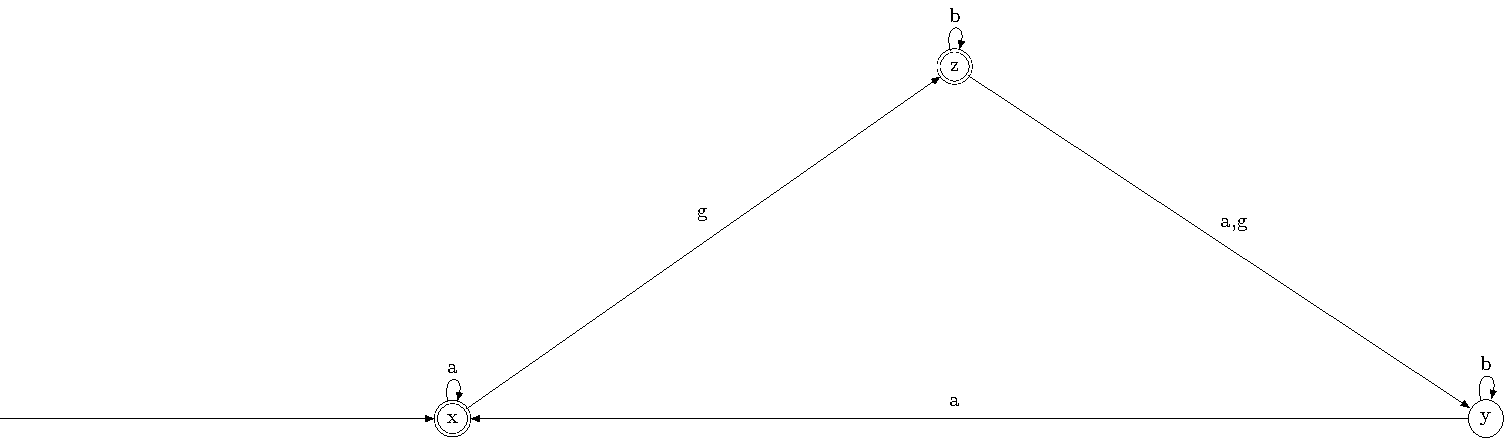
\includegraphics[width=0.8\textwidth]{automata/daoct/example.tikz}
  % \includetikzfigure[width=0.5\textwidth]{automata/example/example}
  \caption{Diagrama de transição de estados para $k=1$.}
  \label{fig:examplek1}
\end{figure}

\end{frame}

\begin{frame}{}
\begin{figure}[H]
    \footnotesize
  \centering 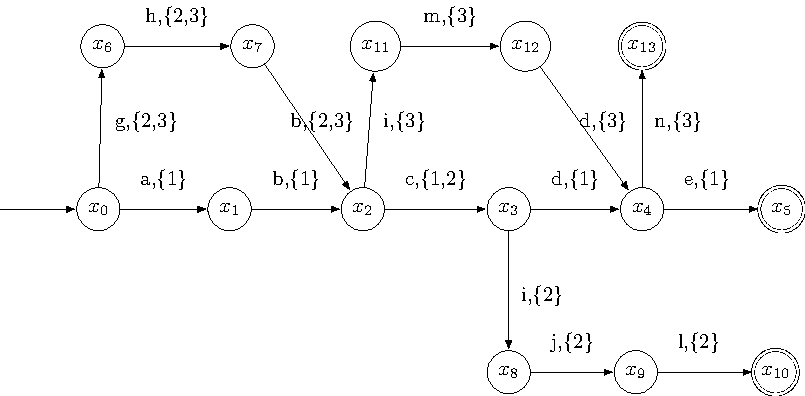
\includegraphics[width=0.9\textwidth]{automata/daoct/examplek2.tikz}
  % \includetikzfigure[width=0.5\textwidth]{automata/example/example}
  \caption{Diagrama de transição de estados para $k=2$.}
  \label{fig:examplek2}
\end{figure}

\end{frame}
\begin{frame}{}
\begin{figure}[H]
  \centering\small
   \sbox0{
\begin{tikzpicture}[scale=0.8]
        % \draw[help lines,xstep=1,ystep=1] (0,0) grid (10,10);
        % \foreach \x in {0,1,...,10} { \node [anchor=north] at (\x,0) {\x}; }
        % \foreach \y in {0,1,...,10} { \node [anchor=east] at (0,\y) {\y}; }
        
        \draw[ultra thick,rounded corners] (3.5,0) rectangle (6.5,1.5);
        \draw[ultra thick,rounded corners] (0.5,2) rectangle (3.5,3.5);
        \draw[ultra thick,rounded corners] (6.5,2) rectangle (9.5,3.5);
        \draw[ultra thick,rounded corners] (3.5,4.5) rectangle (6.5,6);
        \draw (5,5.25) node {Controlador};
        \draw (5,0.75) node {Planta};
        \draw (2,2.75) node {Atuadores};
        \draw (8,2.75) node {Sensores};

        % actuators to plant
        \draw[->,>=stealth, very thick] (2,2) -- (2,0.75) -- (3.5,0.75);

        % controller to actuators
        \draw[->,>=stealth, very thick] (3.5,5.25) -- (2,5.25) -- (2,3.5);

        % Plant to sensors
        \draw[->,>=stealth, very thick] (6.5,0.75) -- (8,0.75) -- (8,2);

        % Sensors to controller
        \draw[->,>=stealth, very thick] (8,3.5) -- (8,5.25) -- (6.5,5.25);

        \draw[->,>=stealth, very thick] (2,4) -- (10,4);
        \draw[fill] (2,4) circle(.05);

        \draw[->,>=stealth, very thick] (8,4.5) -- (10,4.5);
        \draw[fill] (8,4.5) circle(.05);

        \draw (11.4,4.5) node {Sinais};
        \draw (11.4,4.15) node {observavdos};

        % \draw (1.5,5.75) node {Saídas do Controlador};
        % \draw (8.5,5.75) node {Entradas do Controlador};

      \end{tikzpicture}
      }
 \begin{minipage}{1.2\wd0}
  \centering
   \usebox0
  \caption{Sinais Observados de um sistema em malha fechada.}
 \end{minipage}
    \label{fig:obsSignals}
  \end{figure}
\end{frame}


\end{document}

%Examples




%\begin{frame}{Exemplo de frases espaçadas tipo Afonso}
%	\onslide<1,2,3,5>{\quad First Line of Text}
%	\only<2,3>{\\ \quad \quad Second Line of Text}
%	\onslide<3>{\\ \quad \quad \quad Third Line of Text}
%\end{frame}


%\begin{frame}
%\begin{enumerate}
%\item Item 1
%\end{enumerate}
%\begin{itemize}
%\item[\XSolidBrush] Item 1
%\end{itemize}
%\end{frame}
%
%\begin{frame}{Imagem}
%\begin{figure}
%\includegraphics[height=4cm]{redesbr.JPG}
%\caption{Figura}
%\end{figure}
%
%\end{frame}
%
%\begin{frame}{2 images same title}
%\begin{figure}
%   \includegraphics[width=0.475\textwidth]{redesbr.JPG}
%   \hfill
%   \includegraphics[width=0.475\textwidth]{redesbr.JPG}
%   \caption{Imagem tal esquerda e outra direita}
%\end{figure}
%\end{frame}
%
%\begin{frame}{2 images different titles}
%    \begin{figure}[ht]
%        \begin{minipage}[b]{0.45\linewidth}
%            \centering
%            \includegraphics[width=\textwidth]{redesbr}
%            \caption{Label for a}
%            \label{fig:a}
%        \end{minipage}
%        \hspace{0.5cm}
%        \begin{minipage}[b]{0.45\linewidth}
%            \centering
%            \includegraphics[width=\textwidth]{redesbr}
%            \caption{Label for b}
%            \label{fig:b}
%        \end{minipage}
%    \end{figure}
%\end{frame}
%}


